\subsection{Component Fitting}

Component fitting involves modeling the spectral data as a combination of known spectral signatures of soil components. This method allows for the estimation of the concentration of multiple components in the soil based on their spectral contributions.

The combined spectral function is defined as:
\begin{equation}
F_c = \sum_{i} A_i \cdot F_i
\end{equation}

where $F_c$ is the combined spectral function, $A_i$ are the coefficients representing the concentration of each component, and $F_i$ are the spectral functions of individual components.

% \begin{figure}[H]
% \centering
% 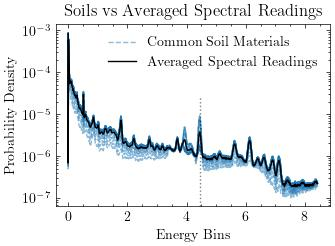
\includegraphics[width=0.8\textwidth]{../Figures/DataGeneration/CommonSoilSpectravsAverageSoilSpectrum.jpg}
% \caption{Common soil spectra vs average soil spectrum showing the spectral signatures of different soil components}
% \label{fig:common_soil_spectra}
% \end{figure}

\begin{figure}[H]
\centering
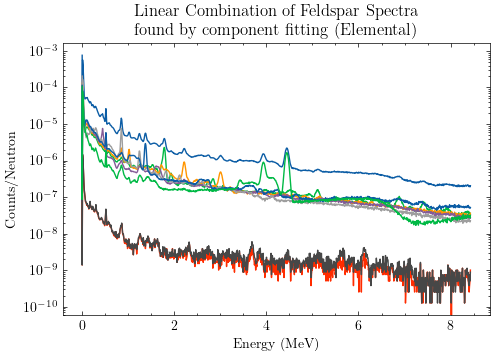
\includegraphics[width=0.8\textwidth]{../Figures/Analysis/elemental_linear_combination_feldspar.png}
\caption{Component fitting process showing linear combination of elemental spectral components for feldspar analysis}
\label{fig:elemental_component_fitting}
\end{figure}

\begin{figure}[H]
\centering
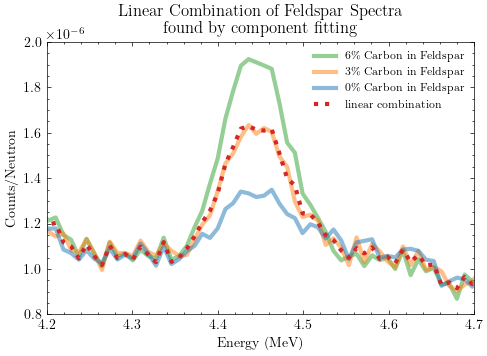
\includegraphics[width=0.8\textwidth]{../Figures/Analysis/linear_combination_feldspar.png}
\caption{Component fitting process showing linear combination of spectral components for feldspar analysis}
\label{fig:component_fitting}
\end{figure}

Components can be any known spectral signature, either from pure elemental samples \cite{kavetskiy_neutron_2023} as shown in figure \ref{fig:elemental_component_fitting} or derived from soil samples similar to the target soil \ref{fig:component_fitting}. The fitting process involves adjusting the coefficients $A_i$ to minimize the difference between the combined spectral function $F_c$ and the observed spectral data. This method also benefits from filtering of low energy signals which are generally more likely to be caused by noise.

The carbon coefficient $A_C$ is then used to estimate the Carbon level in the soil. This method is particularly useful for analyzing complex soil mixtures where multiple known components contribute to the spectral signature. This method is also generalizable to study other elements or compounds.

\begin{figure}[H]
\centering
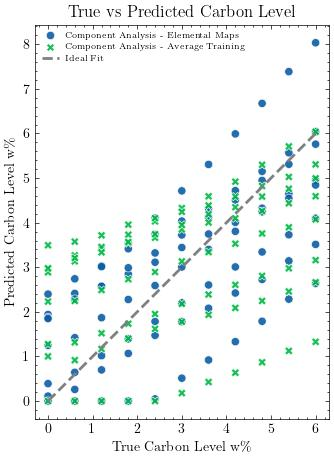
\includegraphics[width=0.8\textwidth]{../Figures/Analysis/carbon_level_vs_predicted_component_analysis.jpg}
\caption{Component fitting prediction results showing carbon level vs predicted values}
\label{fig:component_predictions}
\end{figure}